\chapter{Generating Random WMC Instances}\label{chapter:comparison}

\section{Introduction}

% WMC
Weighted model counting (WMC)---a weighted generalisation of propositional model
counting (\mc{}) \citep{DBLP:journals/ai/ChaviraD08}---has emerged as a powerful
computational framework for problems in a variety of domains. In particular, WMC
has been used to perform probabilistic inference for graphical models such as
Bayesian networks and Markov networks
\citep{DBLP:conf/ecai/BartKLM16,DBLP:conf/ijcai/ChaviraD05,DBLP:conf/sat/ChaviraD06,DBLP:conf/kr/Darwiche02,DBLP:conf/aaai/SangBK05},
probabilistic programs \citep{DBLP:journals/pacmpl/HoltzenBM20}, and
probabilistic logic programs \citep{DBLP:journals/tplp/FierensBRSGTJR15}. More
recently, WMC was used in the context of neural-symbolic artificial intelligence
as well \citep{DBLP:conf/icml/XuZFLB18}. Extensions of WMC add support for
continuous variables \citep{DBLP:conf/ijcai/BellePB15}, infinite domains
\citep{DBLP:conf/aaai/Belle17}, and first-order logic
\citep{DBLP:conf/ijcai/BroeckTMDR11,DBLP:journals/cacm/GogateD16} and generalise
the definition to support arbitrary pseudo-Boolean functions instead of clauses
(\cref{chapter:wmc2}). Exact WMC algorithms can be broadly classified as based
on search \citep{DBLP:conf/sat/SangBBKP04,DBLP:conf/ijcai/SharmaRSM19},
knowledge compilation
\citep{DBLP:conf/ecai/Darwiche04,DBLP:conf/ijcai/LagniezM17,DBLP:conf/ijcai/OztokD15},
and dynamic programming \citep{DBLP:conf/aaai/DudekPV20,DBLP:conf/cp/DudekPV20}.
Other alternatives include approximate \citep{DBLP:conf/aaai/RenkensKBR14} and
parallel algorithms \citep{DBLP:conf/pgm/DalLL18,DBLP:conf/esa/FichteHWZ18},
hybrid approaches \citep{DBLP:conf/sat/HecherTW20}, quantum computing
\citep{DBLP:conf/ecai/Riguzzi20}, and reduction to model counting
\citep{DBLP:conf/ijcai/ChakrabortyFMV15}.

% motivation for the problem
In \cref{chapter:wmc1,chapter:wmc2} as well as recent experimental work by
others
\citep{DBLP:conf/aaai/DudekPV20,DBLP:conf/cp/DudekPV20,DBLP:conf/ijcai/LagniezM17},
we see most WMC algorithms performing very similarly overall but with
overwhelming differences when run on specific subsets of data. Examples of such
segregating data sets include bipartite Bayesian networks by
\citet{DBLP:conf/aaai/SangBK05} and relational Bayesian networks by
\citet{DBLP:journals/ijar/ChaviraDJ06} that encode reachability in graphs under
node deletion. So far, such performance differences remain unexplained. However,
knowledge about the nature of these differences can inform our choices and aid
in further algorithmic developments. Moreover, identifying performance
predictors of algorithms is often an important step in developing a portfolio
approach to the problem \citep{DBLP:journals/jair/XuHHL08}. Lastly, if new
algorithms are always tested on the same set of benchmarks, eventually they may
become somewhat fitted to the particular characteristics of those instances,
leading to algorithms that may perform worse when run on new types of data
\citep{DBLP:conf/cec/HossainALA10}.

% TODO: incorporate this sentence somewhere, referencing the chapter instead.
% Similarly, while there is a recent attempt \citep{DBLP:conf/cp/DilkasB20} to
% compare WMC algorithms on random instances of a particular
% application of WMC (i.e., probabilistic logic programs), it fails to
% discern any meaningful differences among the algorithms.

% related work on SAT
Both theoretical and experimental analysis of SAT (and, to a lesser extent,
\mc{}) algorithms on random instances is a rich area of research spanning almost
forty years. Variations of some of the first random models ever proposed
\citep{DBLP:journals/dam/FrancoP83,DBLP:journals/siamcomp/PurdomB83} continue to
be instrumental up to this day for, e.g., establishing the location of the
threshold between satisfiable and unsatisfiable instances
\citep{DBLP:conf/focs/AchlioptasM02} and efficiently approximating \mc{}
\citep{DBLP:conf/icalp/GalanisG0Y20}. Other random models consider non-uniform
variable frequencies \citep{DBLP:conf/ijcai/AnsoteguiBL09}, fixing the number of
times each variable occurs both positively and negatively
\citep{DBLP:journals/cpc/Coja-OghlanW18}, and adding other constraints such as
cardinality and `exclusive or' \citep{DBLP:conf/ijcai/PoteJM19}. In contrast,
only one WMC algorithm so far has been analysed using random instances
\citep{DBLP:conf/sat/SangBBKP04,DBLP:conf/sat/SangBK05}. The goal of this
chapter is to explain some of the differences between WMC algorithms via an
experimental study that uses random instances.

% parameters for SAT
Experimental work investigating how SAT algorithms behave on random instances is
typically centred around parameters that describe each instance independently of
its size. The most well-known parameter is the ratio of clauses to variables
(i.e., \emph{(clause) density}). Early work in the area showed random 3-SAT
instances to be at their hardest when density is around 4.25
\citep{DBLP:conf/aaai/MitchellSL92}. Later work revealed that the interaction
between density and empirical hardness is much more solver-dependent
\citep{DBLP:journals/constraints/CoarfaDASV03}. Many other parameters such as
heterogeneity, locality, and modularity have emerged from attempts to generate
random instances similar to industry benchmarks for SAT
\citep{DBLP:conf/ijcai/AnsoteguiBL09,DBLP:conf/tacas/BlasiusFS19,DBLP:journals/ai/Giraldez-CruL16,DBLP:conf/ijcai/Giraldez-CruL17}.

% parameters for WMC
What parameter(s) are most appropriate to study WMC\@? Theoretical upper bounds
on the performance of various WMC algorithms typically include a factor
exponential in the primal treewidth of the input formula (or a closely related
notion)
\citep{DBLP:journals/jair/BacchusDP09,DBLP:journals/jacm/Darwiche01,DBLP:conf/ecai/Darwiche04,DBLP:conf/sat/SangBBKP04}.
However---as we show in \cref{sec:model}---instances generated by a standard
random model for $k$-CNF formulas fail to exhibit enough variance in primal
treewidth for us to infer its effect on the behaviour of the algorithms.
Therefore, we present an extension of this model with a parameter that
influences primal treewidth. The performance of WMC algorithms that use data
structures called \emph{algebraic decision diagrams} (ADDs)
\citep{DBLP:journals/fmsd/BaharFGHMPS97} is also known to depend on the
numerical values of weights
\citep{DBLP:conf/aaai/DudekPV20,DBLP:conf/cp/DudekPV20}. Thus, our random model
also includes two parameters that control redundancies in these values. We also
investigate the effect of redundant weight values (e.g., having weights set to
zero and one or having the same weight repeat many times) on the running times
of the algorithms.

In addition to introducing a new random model for WMC instances, the
contributions of this chapter include several key experimental findings about
the behaviour of WMC algorithms---namely,
\textsc{c2d}\footnote{\url{http://reasoning.cs.ucla.edu/c2d/}}
\citep{DBLP:conf/ecai/Darwiche04},
\textsc{Cachet}\footnote{\url{https://cs.rochester.edu/u/kautz/Cachet/}}
\citep{DBLP:conf/sat/SangBBKP04},
\textsc{d4}\footnote{\url{https://www.cril.univ-artois.fr/KC/d4.html}}
\citep{DBLP:conf/ijcai/LagniezM17},
\textsc{DPMC}\footnote{\url{https://github.com/vardigroup/dpmc}}
\citep{DBLP:conf/cp/DudekPV20}, and
\textsc{miniC2D}\footnote{\url{http://reasoning.cs.ucla.edu/minic2d/}}
\citep{DBLP:conf/ijcai/OztokD15}---on random instances. First, we show that the
easy-hard-easy pattern with respect to (w.r.t.) density is different for dynamic
programming algorithms than it is for all other algorithms. Second, we present
statistical evidence that all the algorithms scale exponentially w.r.t.\ primal
treewidth and estimate how the base of that exponential changes w.r.t.\ density.
Third, we show how the performance of ADD-based algorithms gradually improves
w.r.t the proportion of weights that have repeating values and sharply improves
w.r.t.\ the proportion of weights set to zero and one.

% 1. Other parameters include structural entropy
% \cite{DBLP:journals/access/LinWN21}, the proportion of clauses that have at
% most one negative literal has also been suggested as a parameter of
% interest~\cite{DBLP:journals/amai/MaarenN05}.
% 2. Maybe somewhere: relationship between primal treewidth and modularity
% 3. Just like one might choose a different propositional satisfiability
% (SAT) solver based on information about the problem instance at hand (e.g.,
% `is the instance known to be satisfiable?', `was it randomly generated?', `is
% it an industrial instance?')~\cite{DBLP:journals/jair/XuHHL08},
% 4. It was also observed that replacing real numbers with addition and
% multiplication with an arbitrary commutative semiring allows WMC to
% subsume a variety of other problems such as most probable explanation,
% shortest path, and gradient
% computations~\cite{DBLP:journals/ijar/BelleR20,DBLP:journals/japll/KimmigBR17}.
% 5. Having these parameters in the model allows us to look not just at the
% effects of density or primal treewidth on the running times of WMC
% algorithms but also at the interaction between these two parameters of
% interest.

\section{Preliminaries}

% \footnote{Also known by many other names such as Gaifman, (variable)
% interaction, and variable incidence graph.}

By \emph{variable}, we always mean a Boolean variable. A \emph{literal} is
either a variable (say, $v$) or its negation (denoted $\neg v$), respectively
called \emph{positive} and \emph{negative} literal. A \emph{clause} is a
disjunction of literals. A \emph{formula} is any well-formed expression
consisting of variables, negation, conjunction, and disjunction. A formula is in
\emph{conjunctive normal form} (CNF) if it is a conjunction of clauses, and it
is in $k$-CNF if every clause has exactly $k$ literals. While we use the
set-theoretic notation for CNF formulas (e.g., writing $c \in \phi$ to mean that
clause $c$ is one of the clauses in formula $\phi$), duplicate clauses are still
allowed. The \emph{primal graph} of a CNF formula is a graph that has a node for
every variable, and there is an edge between two variables if they coappear in
some clause. The \emph{treewidth} of a graph $G$ measures how similar $G$
is to a tree and is defined as the smallest \emph{width} of any \emph{tree
  decomposition} of $G$ \citep{DBLP:journals/jct/RobertsonS84}. The \emph{primal
  treewidth} of a formula is the treewidth of its primal graph.

Given a CNF formula $\phi$, SAT is a decision problem that asks whether there
exists a way to assign values to all variables in $\phi$ such that $\phi$
evaluates to true. Such a formula is said to be \emph{satisfiable}; otherwise,
it is \emph{unsatisfiable}. \mc{} is a problem that asks to count the number of
such assignments. WMC extends \mc{} with a weight function on literals and asks
to compute the sum of the weights of the models of the given formula, where the
weight of a model is the product of the weights of the literals in it
\citep{DBLP:journals/ai/ChaviraD08}. For example, the WMC of the formula
$x \lor y$ with a weight function
$w\colon \{\,x, y, \neg x, \neg y\,\} \to \mathbb{R}_{\ge 0}$ defined as
$w(x) = 0.3$, $w(y) = 0.2$, $w(\neg x) = 0.7$, $w(\neg y) = 0.8$ is
$w(x)w(y)+w(x)w(\neg y)+w(\neg x)w(y) = 0.3 \times 0.2 + 0.3 \times 0.8 + 0.7 \times 0.2 = 0.44$.

\section{Background on \textsf{\textmd{WMC}} Algorithms}\label{sec:background}

In this section, we briefly review the three major approaches to WMC---search,
knowledge compilation, and dynamic programming---and their corresponding
algorithms. The main search-based WMC algorithm \textsc{Cachet}
\citep{DBLP:conf/sat/SangBBKP04} is based on a conflict-driven clause learning
SAT solver \citep{DBLP:conf/dac/MoskewiczMZZM01}, which is then extended with a
component caching scheme and adapted to counting.

\emph{Knowledge compilation} refers to transformations of propositional formulas
into more restrictive formats that make various operations (such as model
counting) tractable in the size of the representation
\citep{DBLP:journals/jair/DarwicheM02}.
\textsc{c2d} \citep{DBLP:conf/ecai/Darwiche04},
\textsc{d4} \citep{DBLP:conf/ijcai/LagniezM17}, and
\textsc{miniC2D} \citep{DBLP:conf/ijcai/OztokD15}
are all algorithms of this type. \textsc{c2d} compiles to deterministic
decomposable negation normal form
(d-DNNF) \citep{DBLP:journals/jancl/Darwiche01}. Similarly, \textsc{d4} compiles
to decision-DNNF (also known as decomposable decision
graphs) \citep{DBLP:conf/aaai/FargierM06}. The only difference between d-DNNF and
decision-DNNF is that decision-DNNF has if-then-else constructions instead of
disjunctions \citep{DBLP:conf/ijcai/LagniezM17}. Finally,
\textsc{miniC2D} compiles to decision-SDDs---a
subset of sentential decision diagrams (SDDs) that form a subset of
d-DNNF \citep{DBLP:conf/ijcai/Darwiche11}.

All of the algorithms mentioned above execute in exactly the same way regardless
of whether computing WMC or \mc{}. Two recent WMC algorithms instead use data
structures whose size (and thus the runtime of the algorithm) depends on the
numerical values of weights. These data structures are representations of
\emph{pseudo-Boolean functions}, i.e., functions of the form
$f\colon 2^X \to \mathbb{R}_{\ge 0}$, where $X$ is a set, and $2^X$ denotes its
powerset. \textsc{ADDMC} is the first such algorithm
\citep{DBLP:conf/aaai/DudekPV20}. It uses ADDs to represent pseudo-Boolean
functions, combining and simplifying them in a bottom-up dynamic programming
fashion. Since the size of an ADD for $f$ depends on the cardinality of the
range of $f$ \citep{DBLP:journals/fmsd/BaharFGHMPS97}, the performance of the
algorithm is sensitive to the numerical values of weights, e.g., to how
frequently they repeat. \textsc{DPMC} extends \textsc{ADDMC} in two ways
\citep{DBLP:conf/cp/DudekPV20}. First, \textsc{DPMC} allows for the order and
nesting of operations on ADDs to be determined from an
approximately-minimal-width tree decomposition rather than by
heuristics.\footnote{There is also a recent line of work in using tree
  decompositions to guide the heuristics of search-based model counters
  \citep{DBLP:conf/cp/KorhonenJ21}.} Second, tensors are offered as an
alternative to ADDs.

In all known parameterised complexities of WMC algorithms, the exponential
factor is a function of primal treewidth or a closely related parameter.
Interestingly, \textsc{c2d} is specifically designed to handle high primal
treewidth (which the author refers to as \emph{connectivity}
\citep{DBLP:conf/ijcai/Darwiche99}) and improves upon an earlier algorithm that
has $\mathcal{O}(mw2^w)$ time complexity, where $m$ is the number of clauses,
and $w$ is the width of the decomposition tree which is known to be at most
primal treewidth
\citep{DBLP:journals/jacm/Darwiche01,DBLP:conf/ecai/Darwiche04}. While the
complexity of \textsc{Cachet} was not analysed directly, the algorithm is based
on component caching which is known to have a
$2^{\mathcal{O}(w)}n^{\mathcal{O}(1)}$ time complexity, where $n$ is the number
of variables, and $w$ is the branchwidth of the underlying hypergraph
\citep{DBLP:journals/jair/BacchusDP09,DBLP:conf/sat/SangBBKP04}, which is known
to be within a constant factor of primal treewidth
\citep{DBLP:journals/jct/RobertsonS91}. Similarly, the complexity of
\textsf{DPMC} is not described in the paper, although the authors define a
notion of width $w$ that is at most primal treewidth plus one and estimate the
running time of the (execution part of the) algorithm to be proportional to
$2^w$ \citep{DBLP:conf/cp/DudekPV20}.

\section{Random $k$-CNF Formulas with Varying Primal
  Treewidth}\label{sec:model}

\paragraph*{Notation.}
For any graph $G$, we write $\mathcal{V}(G)$ for its set of nodes and
$\mathcal{E}(G)$ for its set of edges. Let $S$ be a finite set. We write
$\mathcal{U}S$ for the discrete uniform probability distribution on $S$. We
represent any other probability distribution as a pair $(S, p)$ where $p\colon S
\to [0, 1]$ is a probability mass function. For any probability distribution
$\mathcal{P}$, we write $x \leftlsquigarrow \mathcal{P}$ to denote the act of
sampling $x$ from $\mathcal{P}$. For instance, $x \leftlsquigarrow (\{\, 1, 2 \,\}, \{\, 1 \mapsto 0.1, 2 \mapsto 0.9 \,\})$ means that $x$ becomes equal to $1$ with probability $0.1$ or to $2$ with probability $0.9$.

Our random model is based on the following parameters:
\begin{itemize}
\item the number of variables $\nu \in \mathbb{N}^+$,
\item density $\mu \in \mathbb{R}_{>0}$,
\item clause width $\kappa \in \mathbb{N}^+$ (for $k$-CNF formulas, $\kappa =
  k$),
\item a parameter $\rho \in [0, 1]$ that influences the primal treewidth of
  the formula,
\item the proportion $\delta \in [0, 1]$ of variables $x$ such that $w(x) = 1$
  and $w(\neg x) = 0$ or $w(x) = 0$ and $w(\neg x) = 1$,
\item and the proportion $\epsilon \in [0, 1-\delta]$ of variables $x$ such that
  $w(x) = w(\neg x) = 0.5$.
\end{itemize}
The first three parameters are the standard parameters used to generate random
$k$-CNF formulas with $\nu\mu$ clauses (up to rounding). We expect to observe
(possibly different) values of $\mu$ that maximize the running time of each
algorithm for fixed values of $\nu$ and $\kappa$. Parameters $\delta$ and
$\epsilon$ control the numerical values of weights and are part of the model
because the running time of \textsc{DPMC} \citep{DBLP:conf/cp/DudekPV20}---and
other algorithms based on ADDs---depends on these values. Weights such as zero
and one are particularly `simplifying' because they are respectively the
additive and multiplicative identities. Having them propagate through the
algorithm reduces the size of many ADDs used by \textsc{DPMC}, making the
algorithm more efficient. Including many copies of the same weight (e.g., 0.5)
can similarly simplify ADDs as well. Other WMC algorithms are indifferent to the
numerical values of weights.

\begin{algorithm}[t]
  \caption{Generating a random formula.}\label{alg:random}
  \SetKwData{kcnf}{kcnf}
  \SetKwFunction{NewVariable}{NewVariable}
  \SetKwProg{Fn}{Function}{:}{}
  \KwIn{$\nu,\kappa \in \mathbb{N}^+$ such that $\kappa < \nu$, $\mu \in
    \mathbb{R}_{>0}$, $\rho \in [0, 1]$.}
  \KwOut{A $k$-CNF formula $\phi$.}
  $\phi \gets \text{empty CNF formula}$\;
  $G \gets \text{empty graph}$\;
  \For{$i \gets 1$ \KwTo $\lfloor \nu\mu \rfloor$}{
    $X \gets \emptyset$\;
    \For{$j \gets 1$ \KwTo $\kappa$}{
      $x \gets \NewVariable{$X$, $G$}$\;
      $\mathcal{V}(G) \gets \mathcal{V}(G) \cup \{\, x \,\}$\;\label{line:7}
      $\mathcal{E}(G) \gets \mathcal{E}(G) \cup \{\, \{\,x, y\,\} \mid y \in X
      \,\}$\;\label{line:8}
      $X \gets X \cup \{\, x \,\}$\;\label{line:9}
    }
    $\phi \gets \phi \cup \{\, l \leftlsquigarrow \mathcal{U}\{\, x, \neg x \,\}
    \mid x \in X \,\}$\;\label{line:construct_clause}
  }
  \Return{$\phi$}\;
  \Fn{\NewVariable{$X$, $G$}}{
    $N \gets \{\, e \in \mathcal{E}(G) \mid |e \cap X| = 1
    \,\}$\;\label{line:13}
    \If{$N = \emptyset$}{
      \Return{$x \leftlsquigarrow \mathcal{U}(\{\, x_1, x_2, \dots, x_\nu \,\}
        \setminus X)$}\;
    }
    \nosemic\Return{$x \leftlsquigarrow \left(\{\, x_1, x_2, \dots, x_\nu \,\}
        \setminus X,\vphantom{\frac{|\{\, z \in X \mid \{\,y, z\,\} \in
            \mathcal{E}(G) \,\}|}{|N|}}\right.$}\;
      \pushline\dosemic$\left. y \mapsto \frac{1 - \rho}{\nu - |X|} +
        \rho\frac{|\{\, z \in X \mid \{\,y, z\,\} \in \mathcal{E}(G)
          \,\}|}{|N|}\right)$\; \label{line:return}
  }
\end{algorithm}

The process behind generating random $k$-CNF formulas is summarized as
\cref{alg:random}. For the rest of this section, let $x_1, x_2, \dots, x_\nu$ be
the variables of the formula under construction. We simultaneously construct
both formula $\phi$ and its primal graph $G$.\footnote{The idea to directly take
  the primal graph into consideration while generating the formula is new---cf.
  random SAT instance generators based on, e.g., adversarial evolution
  \citep{DBLP:conf/cec/HossainALA10} and community structure
  \citep{DBLP:journals/ai/Giraldez-CruL16}.} Each iteration of the first
for-loop adds a clause to $\phi$. This is done by constructing a set $X$ of
variables to be included in the clause, and then randomly adding either $x$ or
$\neg x$ to the clause for each $x \in X$ on \cref{line:construct_clause}.
Function \texttt{NewVariable} randomly selects each new variable $x$, and
\cref{line:7,line:8,line:9} add $x$ to the graph and the formula while also
adding edges between $x$ and all the other variables in the clause. To select
each variable, \cref{line:13} defines set $N$ to contain all edges with exactly
one endpoint in $X$. The edges that will be added to $G$ by \cref{line:8} will
form a subset of $N$. If $N = \emptyset$, we select the variable uniformly at
random (u.a.r.) from all viable candidates. Otherwise, $\rho$ determines how
much we bias the uniform distribution towards variables that would introduce the
smallest number of new edges to $G$.

When $\rho=0$, \cref{alg:random} reduces to what has become the standard random
model for $k$-CNF formulas. Equivalently to \citet{DBLP:journals/dam/FrancoP83},
we independently sample a fixed number of clauses, each clause has no duplicate
variables, and each variable becomes either a positive or a negative literal
with equal probabilities. At the other extreme, when $\rho = 1$, the first
variable of a clause is still chosen u.a.r., but all other variables are chosen
from those that already coappear in a clause (if possible). The probability that
a variable is selected to be included in a clause scales linearly w.r.t.\ the
proportion of edges in $N$ that would be repeatedly added to $G$ if the variable
$y$ was added to the clause. This is an arbitrary choice (which appears to work
well, see \cref{sec:remarks}) although alternatives (e.g., exponential scaling)
could be considered. As long as $\rho < 1$, every $k$-CNF formula retains a
positive probability of being generated by the algorithm.

To transform the generated formula into a WMC instance, we need to define
weights on literals.\footnote{Recall that in \cref{chapter:wmc1,chapter:wmc2} we
  showed that algorithms such as \textsc{DPMC} and \textsc{ADDMC}
  \citep{DBLP:conf/aaai/DudekPV20,DBLP:conf/cp/DudekPV20} become more efficient
  when equipped with a different input format that assigns weights to formulas
  rather than literals.} We want to partition all variables into three groups:
those with weights equal to zero and one, those with weights equal to 0.5, and
those with arbitrary weights, where the size of each group is determined by
$\delta$ and $\epsilon$. To do this, we sample a permutation
$\pi \leftlsquigarrow \mathcal{U}S_\nu$ (where $S_\nu$ is the permutation group
on $\{1, 2, \dots, \nu \}$), and assign to each \emph{variable} $x_n$ a weight
drawn u.a.r.\ from
\begin{itemize}
\item $\mathcal{U}\{\,0, 1\,\}$ if $\pi(n) \le \nu\delta$,
\item $\mathcal{U}\{\,0.5\,\}$ if $\nu\delta < \pi(n) \le \nu\delta +
  \nu\epsilon$,
\item and $\mathcal{U}\{\, 0.01, 0.02, \dots, 0.99 \,\}$\footnote{For
    convenience, we represent $(0, 1)$ as 99 discrete values.} if $\pi(n) >
  \nu\delta + \nu\epsilon$.
\end{itemize}
We extend these weights to weights on \emph{literals} by choosing the weight of
each positive literal to be equal to the weight of its variable, and the weight
of each negative literal to be such that $w(x) + w(\neg x) = 1$ for all
variables $x$. This restriction is to ensure consistent answers among the
algorithms.

\begin{example}\label{example:algorithm}
  Let $\nu = 5$, $\mu = 0.6$, $\kappa = 3$, $\rho = 0.3$, $\delta = 0.4$,
  and $\epsilon = 0.2$ and consider how \cref{alg:random} generates a random
  instance. Since $\kappa = 3$, and $\lfloor\nu\mu\rfloor = 3$,
  the algorithm will generate a 3-CNF formula with three clauses.

  For the first variable of the first clause, we are choosing u.a.r.\ from $\{\,
  x_1, x_2, \dots, x_5 \,\}$. Suppose the algorithm chooses $x_5$. Graph $G$
  then gets its first node but no edges. The second variable is chosen u.a.r.
  from $\{\, x_1, x_2, x_3, x_4 \,\}$. Suppose the second variable is $x_2$.
  Then $G$ gets another node and its first edge between $x_2$ and $x_5$. The
  third variable in the first clause is similarly chosen u.a.r.\ from $\{\, x_1,
  x_3, x_4 \,\}$ because the only edge in $G$ has both endpoints in $X = \{\,
  x_2, x_5 \,\}$, and so $N = \emptyset$. Suppose the third variable is $x_1$.
  Graph $G$ becomes a triangle connecting $x_1$, $x_2$, and $x_5$. Each of
  the three variables is then added to the clause as either a positive or a
  negative literal (with equal probabilities). Thus, the first clause becomes,
  e.g., $\neg x_5 \lor x_2 \lor x_1$.

  The first variable of the second clause is chosen u.a.r.\ from $\{\, x_1, x_2,
  \dots, x_5\,\}$. Suppose it is $x_5$ again. When the function
  \texttt{NewVariable} tries to choose the second variable, $X = \{\, x_5 \,\}$,
  and so $N = \{\, \{\, x_1, x_5 \,\}, \{\, x_2, x_5 \,\}\,\}$. The second
  variable is chosen from the discrete probability distribution
  \[
    \Pr(x_1) = \Pr(x_2) = \frac{1 - 0.3}{5 - 1} + 0.3 \times \frac{1}{2} = 0.325
  \]
  and
  \[
    \Pr(x_3) = \Pr(x_4) = \frac{1 - 0.3}{5 - 1} = 0.175.
  \]

  We skip the details of how all remaining variables and clauses are selected
  and consider the weight assignment. First, we shuffle the list of variables
  and get, e.g., $L = (x_4, x_3, x_2, x_1, x_5)$. This means that the first
  $\nu\delta = 5 \times 0.4 = 2$ variables of $L$ get weights u.a.r.\ from $\{\,
  0, 1 \,\}$, the next $\nu\epsilon = 5 \times 0.2 = 1$ variable gets a weight
  of 0.5, and the remaining two variables get weights u.a.r.\ from $\{\,0.01,
  0.02, \dots, 0.99 \,\}$. The weight function $w\colon \{\, x_1, x_2, \dots,
  x_5, \neg x_1, \neg x_2, \dots, \neg x_5\,\} \to [0, 1]$ can then be defined
  as, e.g., $w(x_4) = w(\neg x_3) = 0$, $w(x_3) = w(\neg x_4) = 1$, $w(x_2) =
  w(\neg x_2) = 0.5$, $w(x_1) = 0.23$, $w(\neg x_1) = 0.77$, $w(x_5) = 0.18$,
  and $w(\neg x_5) = 0.82$.
\end{example}

% \begin{remark}
%   Note that not having a parameter that in some way influences primal treewidth
%   is unrealistic for generating instances with a wide range of primal treewidth
%   values. Without such a parameter (i.e., if $\rho=0$), the variance of primal
%   treewidth is relatively small compared to the range of values one could
%   generate by varying $\rho$ between zero and one (evidence for this is in
%   \cref{sec:remarks}).
% \end{remark}

% If all weights are different real numbers in $(0, 1)$, then performing
% addition and multiplication on them is unlikely to result in any duplicates,
% and the number of nodes in ADDs is maximised.

% i.e., the permutation $\pi$ is
% \[
%   \pi =
%   \begin{pmatrix}
%     1 & 2 & 3 & 4 & 5\\
%     4 & 3 & 2 & 1 & 5
%   \end{pmatrix}
% \]

% The novel part of the algorithm is centred around \cref{line:return}.

\subsection{Validating the Model}\label{sec:remarks}

The idea behind our model is that manipulating the value of $\rho$ should allow
us to generate instances of varying primal treewidth. Is this effect observable
in practice? In addition, as WMC instances are mostly used for probabilistic
inference, they tend to be satisfiable. Therefore, we want to filter out
unsatisfiable instances from those generated by the model and need to ensure
that the proportion of satisfiable instances remains sufficiently high. Given
that higher values of $\rho$ can result in constraints on variables being more
localised and concentrated, we ask: are instances generated with higher values
of $\rho$ less likely to be satisfiable? To answer both questions, we run the
following experiment.

\begin{experiment}\label{exp:regular_satisfiability}
  We fix $\nu = 100, \delta = \epsilon = 0$, and consider random instances with
  $\mu = 2.5 \times \sqrt{2}^{-5}, 2.5 \times \sqrt{2}^{-4}, \dots, 2.5 \times
  \sqrt{2}^5$, $\kappa = 2, 3, 4, 5$, and $\rho$ going from 0 to 1 in steps of
  0.01. For each combination of parameters, we generate ten instances.\footnote{Since one expects similar values of $\rho$ to produce instances with similar properties, and $\rho$'s are enumerate quite densely, generating only ten instances is sufficient.} We check if each instance is satisfiable using \textsc{MiniSat}\footnote{\url{http://minisat.se/MiniSat.html}}~2.2.0 \citep{DBLP:conf/sat/EenS03} and calculate its (approximate) primal treewidth using \textsc{htd}\footnote{\url{https://github.com/mabseher/htd}} \citep{DBLP:conf/cpaior/AbseherMW17}.
\end{experiment}

\begin{figure}[t]
  \centering
  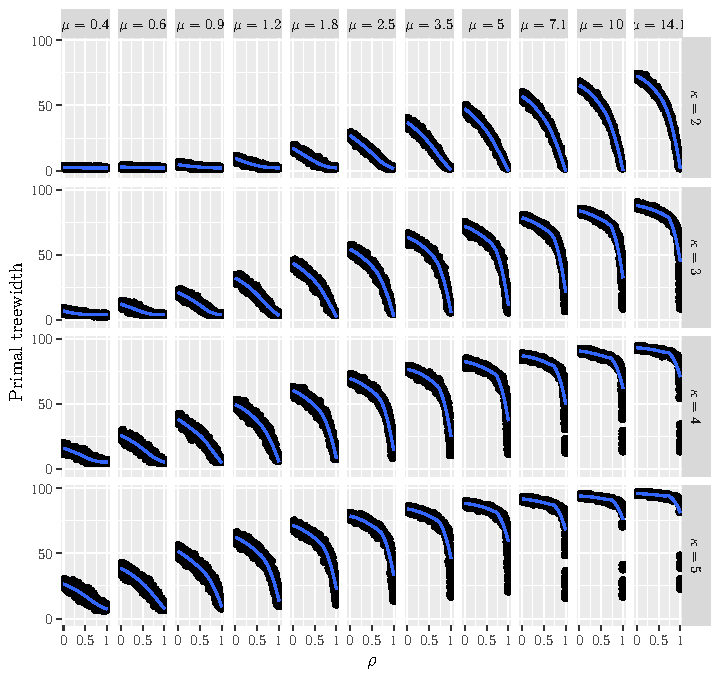
\includegraphics{chapters/comparison/regular_repetitiveness.pdf}
  \caption{The relationship between $\rho$ and primal treewidth for various
    values of $\mu$ and $\kappa$ for $k$-CNF formulas from
    \cref{exp:regular_satisfiability}. Black points represent individual
    instances, and blue lines are smoothed means computed using locally weighted
    smoothing. The values of $\mu$ are rounded to one decimal
    place.}\label{fig:regular_repetitiveness}
\end{figure}

\Cref{fig:regular_repetitiveness} shows the relationship between $\rho$ and
primal treewidth. Except for when both $\mu$ and $\kappa$ are set to very low
values (i.e., the formulas are small in both clause width and the number of
clauses), primal treewidth decreases as $\rho$ increases. This downward trend
becomes sharper as $\mu$ increases, however, not uniformly: it splits into a
roughly linear segment that approaches a horizontal line (for most values of
$\rho$) and a sharply-decreasing segment that approaches a vertical line (when
$\rho$ is close to one). Higher values of $\kappa$ seem to expedite this
transition, i.e., with a higher value of $\kappa$, a lower value of $\mu$ is
sufficient for a smooth downward curve between $\rho$ and primal treewidth to
turn into a combination of a horizontal and a vertical line. While this
behaviour may be troublesome when generating formulas with higher values of
$\mu$ (almost all of which would be unsatisfiable), the relationship between
$\rho$ and primal treewidth is excellent for generating 3-CNF formulas close to
and below the satisfiability threshold of
4.25 \citep{DBLP:journals/ai/CrawfordA96}.

Regarding satisfiability, the proportion of satisfiable 3-CNF formulas drops
from \SI{63.6}{\percent} when $\rho = 0$ to \SI{50.9}{\percent} when $\rho = 1$,
so---while $\rho$ does affect satisfiability---the effect is not significant
enough to influence our experimental setup in the next section.

% It is well-known that there is a sharp transition from satisfiable to
% unsatisfiable 3-CNF formulas at $\mu = 4.25$ regardless of the value of $\nu$
% (this is known as the \emph{satisfiability
% threshold})~\cite{DBLP:journals/ai/CrawfordA96}.

\section{Experimental Results}\label{sec:experiments}

\begin{figure}[t]
  \centering
  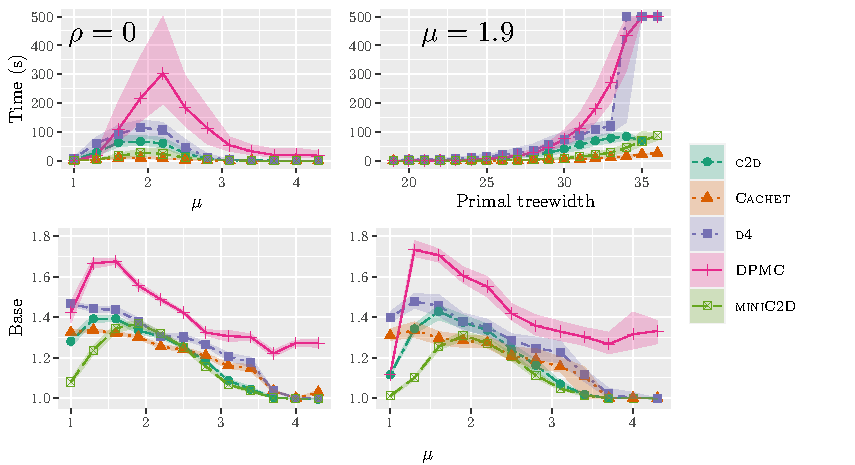
\includegraphics{chapters/comparison/treewidth}
  \caption[Visualisations of the data from \cref{exp:density}. The top-left plot
  shows how the running time of each algorithm changes w.r.t.\ density when
  $\rho = 0$. The top-right plot shows changes in the running time of each
  algorithm w.r.t.\ primal treewidth with $\mu$ fixed at $1.9$. The plots at the
  bottom show how the estimated base of the exponential relationship between
  primal treewidth and the runtime of each algorithm depends on $\mu$. The
  bottom-left plot is for the simple linear model (with shaded regions showing
  standard error), and the bottom-right plot uses the estimates provided by ESA
  (with shaded regions showing \SI{95}{\percent} confidence intervals).]%
  {Visualisations of the data from \cref{exp:density}. The top-left plot shows
    how the running time of each algorithm changes w.r.t.\ density when
    $\rho = 0$. The top-right plot shows changes in the running time of each
    algorithm w.r.t.\ primal treewidth with $\mu$ fixed at $1.9$. The plots at
    the bottom show how the estimated base of the exponential relationship
    between primal treewidth and the runtime of each algorithm depends on $\mu$.
    The bottom-left plot is for the simple linear model (with shaded regions
    showing standard error), and the bottom-right plot uses the estimates
    provided by ESA \protect{\citep{DBLP:conf/gecco/PushakH20}} (with shaded
    regions showing \SI{95}{\percent} confidence intervals).}\label{fig:treewidth}
\end{figure}

% the experimental setup
In this section, we describe three experiments that examine how the running
times of WMC algorithms change w.r.t.\ parameters of our random model. All
experiments were run on Intel Xeon~E5--2630 with Scientific Linux~7, GCC~10.2.0,
Python~3.8.1, R~4.1.0, \textsc{c2d}~2.20 \citep{DBLP:conf/ecai/Darwiche04},
\textsc{Cachet}~1.22 \citep{DBLP:conf/sat/SangBBKP04}, \textsc{htd}~1.2.0
\citep{DBLP:conf/cpaior/AbseherMW17}, and with no additional preprocessing. With
both \textsc{c2d} and \textsc{d4}, we use
\textsc{query-dnnf}\footnote{\url{http://www.cril.univ-artois.fr/kc/d-DNNF-reasoner.html}}
to compute the numerical answer from the compiled circuit. We omit
\textsc{ADDMC} \citep{DBLP:conf/aaai/DudekPV20} from our experiments as it
exceeds time and memory limits on too many instances; however, observations
about the behaviour of \textsc{DPMC} \citep{DBLP:conf/cp/DudekPV20} apply to
\textsc{ADDMC} as well, with the addendum that the tree decomposition implicitly
used by \textsc{ADDMC} may have a significantly higher width. \textsc{DPMC} is
run with tree decomposition-based planning (using one iteration of \textsc{htd})
and ADD-based execution---the combination that was originally found to be most
effective. We restrict our attention to 3-CNF formulas, generate 100 satisfiable
instances for each \emph{combination} of parameters, and run each of the five
algorithms with a \SI{500}{\second} time limit and an \SI{8}{\gibi\byte} memory
limit. While both limits are somewhat low, we prioritise large numbers of
instances to increase the accuracy and reliability of our results. Unless stated
otherwise, in each plot of this section, lines denote median values, and shaded
regions show interquartile ranges. We run the following three experiments,
setting $\nu = 70$ in all of them as we found that this produces instances of
suitable difficulty.

\begin{experiment}[Density and Primal Treewidth]\label{exp:density}
  Let $\nu = 70$, $\mu$ go from 1 to 4.3 in steps of 0.3, $\rho$ go from 0 to
  0.5 in steps of 0.01, and $\delta = \epsilon = 0$.
\end{experiment}

\begin{experiment}[$\delta$]\label{exp:delta}
  Let $\nu = 70$, $\mu = 2.2$\footnote{\Cref{exp:density} shows this density to
    be the most challenging for \textsc{DPMC}.},
  $\rho = 0$, $\delta$ go from 0 to 1 in steps of 0.01, and $\epsilon = 0$.
\end{experiment}

\begin{experiment}[$\epsilon$]\label{exp:epsilon}
  Same as \cref{exp:delta} but with $\delta = 0$ and $\epsilon$ going from 0 to
  1 in steps of 0.01.
\end{experiment}

% c2d and d4 are the most memory-hungry
In each experiment, the proportion of algorithm runs that timed out never
exceeded \SI{3.8}{\percent}. While in \cref{exp:density} only \SI{1}{\percent}
of experimental runs ran out of memory, the same percentage was higher in
\cref{exp:delta,exp:epsilon}---10 and \SI{12}{\percent}, respectively.
\textsc{d4} \citep{DBLP:conf/ijcai/LagniezM17} and
\textsc{c2d} are the algorithms that
experienced the most issues fitting within the memory limit, accounting for
\SIrange{66}{72}{\percent} and \SIrange{28}{33}{\percent} of such instances,
respectively. We exclude the runs that terminated early due to running out of
memory from the rest of our analysis.

% Peaks w.r.t. density: DPMC different from other WMC algorithms which are
% different from #SAT algorithms
In \cref{exp:density}, we investigate how the running time of each algorithm
depends on the density and primal treewidth by varying both $\mu$ and $\rho$.
The results are in \cref{fig:treewidth}. The first thing to note is that the
peak hardness w.r.t.\ density occurs at around 1.9 for all algorithms except for
\textsc{DPMC}, which peaks at 2.2 instead.\footnote{While exact values might be
  hard to read from the plot, they are confirmed by numerical data.} This
finding is consistent with previous work, which shows \textsc{Cachet} to peak at
1.8 \citep{DBLP:conf/sat/SangBBKP04}.\footnote{For comparison, \mc{} algorithms
  have been observed to peak at densities 1.2 and 1.5
  \citep{DBLP:conf/aaai/Pehoushek00}.}

\begin{figure}[t]
  \centering
  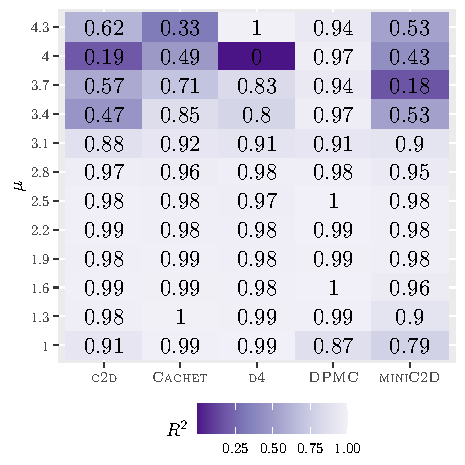
\includegraphics{chapters/comparison/r2}
  \caption{The coefficients of determination (rounded to one decimal place) of
    all the linear models fitted for the top-right subplot of
    \cref{fig:treewidth}.}\label{fig:r2}
\end{figure}

\begin{figure}[t]
  \centering
  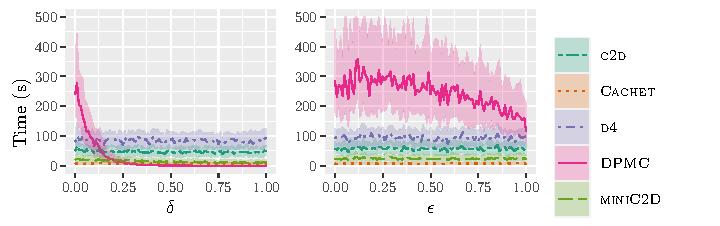
\includegraphics{chapters/comparison/delta_epsilon}
  \caption{Changes in the running time of each algorithm as a result of changing
    $\delta$ (on the left-hand side) and $\epsilon$ (on the right-hand side)
    according to the data from
    \cref{exp:delta,exp:epsilon}.}\label{fig:delta_epsilon}
\end{figure}

The other question we want to investigate using this experiment is how each
algorithm scales w.r.t.\ primal treewidth. The top-right plot in
\cref{fig:treewidth} shows this relationship for a fixed value of $\mu$, and one
can see some evidence that the running time of \textsc{DPMC} grows faster
w.r.t.\ primal treewidth than the running time of the other algorithms. We use
two statistical techniques to quantify this growth: a simple linear regression
model and the empirical scaling analyzer
(ESA)~v2\footnote{\url{https://github.com/YashaPushak/ESA}}
\citep{DBLP:conf/gecco/PushakH20}. In both cases, for each algorithm and value
of $\mu$ in \cref{exp:density}, we select the median runtime for all available
values of primal treewidth. In the former case, we fit the model
$\ln t \sim \alpha w + \beta$, where $t$ is the median running time of the
algorithm, $w$ is the primal treewidth, and $\alpha$ and $\beta$ are
parameters.\footnote{Similar statistical analyses have been used to investigate
  polynomial-to-exponential phase transitions in SAT
  \citep{DBLP:journals/constraints/CoarfaDASV03} and the behaviour of SAT
  solvers on CNF-XOR formulas \citep{DBLP:conf/ijcai/DudekMV17}.} In other
words, this model attempts to express median running time as
$e^\beta{(e^\alpha)}^w$. In the latter case, we run ESA with 1001 bootstrap
samples, a window of 101, and use the first \SI{30}{\percent} of the data for
training.

% DPMC scales worse w.r.t. primal treewidth (across all densities)
The results of both models are qualitatively the same (with the exception of
\textsc{DPMC} run on instances with $\mu = 1$) and are displayed at the bottom
of \cref{fig:treewidth}. We find that, indeed, \textsc{DPMC} scales worse
w.r.t.\ primal treewidth than any other algorithm across all values of $\mu$ and
is the only algorithm that does not become indifferent to primal treewidth when
faced with high-density formulas. A second look at the top-left subplot of
\cref{fig:treewidth} suggests an explanation for the latter observation. The
running times of all algorithms except for \textsc{DPMC} approach zero when
$\mu > 3$ while the median running time of \textsc{DPMC} approaches a small
non-zero constant instead. This observation also explains why \cref{fig:r2}
shows that the fitted models fail to explain the data for non-ADD algorithms
running on high-density instances---the running times are too small to be
meaningful. In all other cases, an exponential relationship between primal
treewidth and runtime fits the experimental data remarkably well.

% miniC2D is good at low-density high-primal-treewidth instances
Another thing to note is that \textsc{miniC2D} \citep{DBLP:conf/ijcai/OztokD15}
is the only algorithm that exhibits a clear low-high-low pattern in the bottom
subplots of \cref{fig:treewidth}. To a smaller extent, the same may apply to
\textsc{c2d} and \textsc{DPMC} as well, although the evidence for this is
limited due to relatively large gaps between different values of $\mu$ in
\cref{exp:density}. In contrast, the running times of \textsc{Cachet} and
\textsc{d4} remain dependent on primal treewidth even when the density of the
WMC instance is very low, suggesting that \textsc{miniC2D} should have an
advantage on low-density high-primal-treewidth instances.

% A median instance with all weights equal to 0.5 is about three times easier
% than a median instance with completely random weights.
Finally, \cref{exp:delta,exp:epsilon} investigate how changing the numerical
values of weights can simplify a WMC instance. The results are in plotted
\cref{fig:delta_epsilon}. As expected, the running time of all algorithms other
than \textsc{DPMC} stay the same regardless of the value of $\delta$ or
$\epsilon$. The running time of \textsc{DPMC}, however, experiences a sharp
(exponential?) decline with increasing $\delta$. The decline w.r.t. $\epsilon$
is also present, although significantly less pronounced and with high variance.

How are these random instances different from real data? As a representative
sample, we take the WMC encodings of Bayesian networks created using the method
by \citet{DBLP:conf/aaai/SangBK05} as found in the experimental
setup\footnote{\url{https://github.com/vardigroup/DPMC/releases}} of the
\textsc{DPMC} paper \citep{DBLP:conf/cp/DudekPV20}. A typical WMC instance has
$\nu = 200$ variables, half of which have equal weights (i.e.,
$\epsilon = 0.5$), an average clause width of $\kappa = 2.6$, a density of
$\mu = 2.5$, and a primal treewidth of 28. Our random instances have fewer
variables and (for the most part) lower density. Another important difference is
that our instances are in $k$-CNF whereas a typical encoding of a Bayesian
network has many two-literal clauses mixed with clauses of various longer
widths. Despite real instances having more variables, their primal treewidth is
rather low. Perhaps this partially explains why the performance of \textsc{DPMC}
is in line with the performance of all other algorithms on traditionally-used
benchmarks \citep{DBLP:conf/cp/DudekPV20} despite struggling with most of our
random data.

To sum, we found that \textsc{c2d} and \textsc{d4} are the most memory-intensive
algorithms, \textsc{Cachet} is great on random instances in general,
\textsc{miniC2D} exceeds on low-density high-primal-treewidth instances, and
\textsc{DPMC} is at its best on low-density low-primal-treewidth instances.
Furthermore, a median instance with all weights equal to each other is about
three times easier for \textsc{DPMC} than a median instance with random weights.
Another important observation is about how peak hardness w.r.t.\ density depends
on the algorithm: \textsc{DPMC} peaks at a higher density than all other WMC
algorithms, which peak at a higher density than (some) \mc{} algorithms.

\section{Conclusions and Future Work}

In this chapter, we studied the behaviour of and differences among WMC
algorithms on random instances generated by a standard model for $k$-CNF
formulas extended with parameters that control primal treewidth and literal
weights. Among other things, we established statistical evidence for the
existence of an exponential relationship between primal treewidth and the
running time of all WMC algorithms. The running time of ADD-based algorithms was
observed to peak at a higher density, scale worse w.r.t.\ primal treewidth, and
depend negatively on repeating weight values compared to algorithms based on
search or knowledge compilation. These observations can, to some degree, be
extended to a closely related weighted projected model counting algorithm
\citep{DBLP:conf/sat/DudekPV21} as well as to other applications of ADDs more
generally, e.g., probabilistic inference
\citep{DBLP:conf/ijcai/ChaviraD07,DBLP:conf/uai/GogateD11} and stochastic
planning \citep{DBLP:conf/uai/HoeySHB99}.

One limitation of our work is that variability in primal treewidth was achieved
via a parameter, and this could bias randomness in some unexpected way (although
it is encouraging that there is only a slight decrease in the proportion of
satisfiable instances between $\rho=0$ and $\rho = 1$). Perhaps a theoretical
investigation of the proposed model is warranted, including a characterisation
of how $\rho$ influences primal treewidth and the structure of the primal graph
more generally. Since treewidth is widely used in parameterised complexity
\citep{DBLP:series/txcs/DowneyF13}, formally establishing a connection with
$\rho$ could make our random model useful for a variety of other hard
computational problems.

To keep the number of experiments feasible, we restricted our attention to 3-CNF
formulas, although, of course, this is not very representative of real-world WMC
instances. The model could be adapted to generate non-$k$-CNF formulas, and
perhaps a more representative structure could be achieved by introducing new
variables that clauses define to be equivalent to select conjunctions of
literals as is done in one of the WMC encodings for Bayesian networks
\citep{DBLP:conf/kr/Darwiche02}.

% It would also be interesting to see whether WMC
% algorithms differ in their ability to effectively handle a `shattered' solution
% space, where most solutions are distant to each other w.r.t. the Hamming
% distance \cite{DBLP:journals/rsa/AchlioptasCR11,DBLP:conf/ijcai/DudekMV17}.
